\documentclass[border={-30pt -10pt -30pt -10pt}]{standalone}
\usepackage{pgfplots}
\usepackage{tikz}

\begin{document}

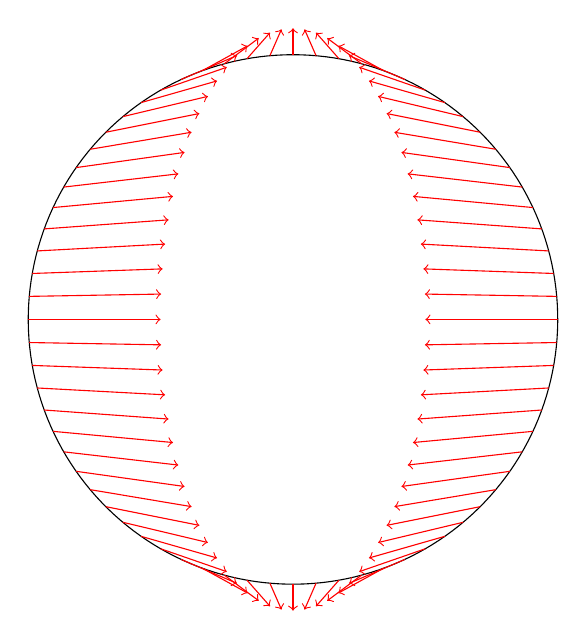
\begin{tikzpicture}
  \begin{axis}[axis lines=none, axis equal,
    width=1\textwidth,
    xmin=6,xmax=10,
    ]
    \addplot[domain=0:360,samples=200]({7 +1 +
      2*sin(x)},{2*cos(x)});

    \foreach \q in {1,...,72}
    \addplot[->, red, domain=0:2.5,samples=5]
    ({7 + (1-(1-x /5)*sin(\q *5)*2},
    {(1 + x /25)*2*cos(\q *5)});
  \end{axis}
\end{tikzpicture}

\end{document}